% TODO: Update these numbers when we are given new datasets.
\section{Data} \label{sec:data}

As described earlier we use data from the Danish company MaCom. The dataset
provided by MaCom is a file consisting of set of texts in Danish where each text
is associated with an author ID. We have been given several text extractions
of different sizes with the biggest dataset consisting of 32,682 texts. The
dataset consist of texts of many different sizes. The shortest text consist of 2
characters and the longest text of 1,849,919 characters. The average length of
each text is 5689 characters with a median of 5363 characters. That means that
almost all texts is close to the average and only a few has sizes much greater
or smaller than the average. The dataset contains 2047 different authors with
an average of 16 texts. The author with the smallest amount of text has two
texts and the author with the most amount of text has 33 texts.

In several of our experiments we limited the number of different characters
we represented. We did that to simplify the amount of different characters
our neural networks had to consider. In particular we cutoff any characters
that occurred with a frequency less than $\frac{1}{100.000}$. We wanted to
make sure that the cutoff only removed characters that were so infrequent
that it would be hard for the neural networks to learn anything from them.
Since the average amount of characters in a single text were 5851 characters
most texts wont include any character that has a frequency below the above
cutoff point. While we wanted to limit the number of different characters
the network would have to consider we also wanted to make sure that a couple
of Danish characters would be considered. In particular the characters \ae,
\o, \aa, \AE, \O\ and \AA. Those characters occur with the frequencies
$7.23\cdot10^{-3}$, $5.5\cdot10^{-3}$, $8.5\cdot10^{-3}$, $1.85\cdot10^{-5}$,
$3.13\cdot10^{-5}$ and $2.08\cdot10^{-5}$ respectively and will therefore
all be included. The overall frequency distribution can be seen in figure
\ref{fig:character_frequencies}.

\begin{figure}[htb]
    \centering
    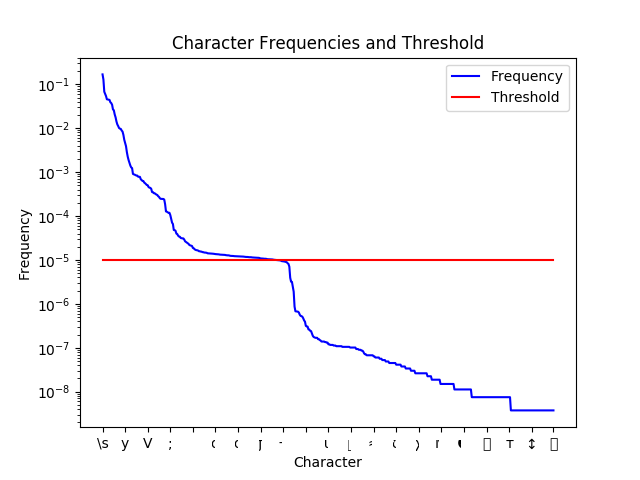
\includegraphics[scale=.8]{./pictures/data/character_frequencies.png}
    \caption{The frequency distribution of characters in the training dataset,
        only a random subset of characters is shown on the x-axis, including the
        most and least frequent. The most frequent character is a space
        character which is why the place is empty.}
    \label{fig:character_frequencies}
\end{figure}

In addition to limiting the characters based on their frequency, we also chose
to limit the overall character count. This was a result of looking at the
character count statistics listed in the beginning of this section. The texts
which had only a very small character count compared to the average and median,
was in most cases just a blank assignment submission. A blank submission, is
when a student doesn't provide an text, as their submission, but rather a
document containing nothing, or a declaration of them not having produced a
text. As such the existence of these papers wont yield any positive input to our
applied method, and is therefore removed. This is done by applying a 200 minimum
character limit on each text in our data, which resulted in 356 being removed
from out dataset. On the other hand a character count which is too large, can
also negatively impact the application of our different methods. This isn't
necessarily tied to the content of the text, but rather the count. When applying
our deep learning methods, all texts are padded to match the longest on in the
data set. This means that in our case, all texts would have to padded to match
the character count of 1,849,919. This would lead to a very large decrease in
performance, with the only payoff being that we would get to keep the large
outlier in our data set. We didn't believe that this trade-off was worth it,
so we applied a 30.000 character upper limit on our data set. In the end, this
resulted in only 12 texts being ignored.

On the topic of erroneous extracts, the texts we were given were extracted from
\textit{.pdf} files and there will therefore sometimes be garbage included. In
order to combat that, we looked at the average unique character count of each of
the texts in the data set. They had an average of of 59 unique characters, and
a median of 61 unique characters. Comparing this to the fact that the minimum
unique character count is 2, and the max unique character count is 280,
left us to deduce that there was some outliers in the set in terms of unique
character count. After looking at the texts with the highest unique character
count, a trend emerged. If a text had over around 100 characters, the text
mostly contained garbage characters. A result from a erroneous data extraction.
These texts also contained and abnormally large character count, and as such
was removed by out 30.000 character limit. In total there were only around 5 of
these texts, so the impact on overall data integrity was negligible. While 100
seems as quite a forgiving threshold compared to the average and the median, the
texts under that threshold had a large unique character count, due to the usage
of different languages, containing character from other alphabets. This caused a
elevation of unique characters used. However the addition of these new character
wont have an impact on the data integrity either, due to the $\frac{1}{100.000}$
frequency threshold described earlier.
